\documentclass[a4paper,openany,12pt]{book}
\usepackage{graphicx}
\usepackage[spanish,mexico]{babel}
\usepackage{fancyhdr}
\usepackage{ae}
\usepackage[left=2.5cm,right=2.5cm,top=3cm,bottom=2cm]{geometry}
\usepackage[printonlyused]{acronym}
\usepackage{xspace}
\usepackage{hlundef}
\usepackage{tesis}
\usepackage{setspace}
\usepackage{algorithm}
\usepackage{algorithmicx}
\usepackage{algpseudocode}
\usepackage{amsmath}
\usepackage{amssymb}
\usepackage{pgfplots}
\usepackage{tabularx}

\title{T�tulo de la Tesis}

\author{Jos� Carlos Delgado Ramos}

\advisor{Prof Dr. Yv�n Jes�s T�pac Valdivia}

\examinerone{Prof. Dr. Alex Jes�s Cuadros Vargas}{Presidente}%
\examinertwo{Prof. Dr. Juan Carlos Guti�rrez C�ceres}{Secretario}%
\examinerthree{Prof. Dr. Jos� Eduardo Ochoa Luna}{Integrante}%
%\examinerfour{Prof. Dr. Yv�n Jes�s T�pac Valdivia}{Externo}{Universidad del ABC} % of being the case
\date{08 de Diciembre de 2014}
\date{\today}

\dedicado{\textit{You have nothing to do but mention the quantum theory, and people will take your voice for the voice of science, and believe anything} \\ George Bernard Shaw (1938)}

\begin{document}
\pagestyle{fancy}

\maketitle %Compone la car�tula y la dedicatoria
\newpage

%Compone la hoja de firmas de los asesores
%\approved{\tres}%  {\tres} or {\cuatro}

%mayores detalles de como usas las abreviaturas (acronimos)
% vea: http://www.ctan.org/tex-archive/macros/latex/contrib/acronym/
% hay un manual en pdf en esa misma direccion

\chapter*{Abreviaturas}

\begin{acronym}
\acro{SPC}{Sociedad Peruana de Computaci�n}
\acro{CMM}{\textit{Capability Maturity Model}}
\end{acronym}


%\begin{agradecimientos}
Aqu� deber�s colocar a quien y porque agradeces. Ejemplo:

En primer lugar deseo agradecer a Dios por haberme guiado a lo largo de estos cinco a�os de estudio.

Agradezco a mis padres por el apoyo brindado para forjarme como un profesional.

Agradezco a la universidad, mi \textit{alma matter}, por haberme cobijado y brindado la formaci�n que ahora me permitir� ayudar a construir una mejor sociedad.

Agradezco de forma muy especial a mi orientador Prof. Dr./Mag. nombre 1 por haberme guiado en esta tesis. ...

Deseo agradecer de forma especial a mis docentes: nombre 1, nombre 2, nombre 3 porque fueron ejemplos que deseo seguir en mi vida profesional.

Deseo agradecer al personal administrativo de la universidad: nombre 1, nombre 2, nombre 3. Muchas gracias por la atenci�n brindada y porque siempre estuvieron dispuestas a ayudarnos.
\end{agradecimientos}
 %Inserta los agradecimientos
\begin{abstract}

This thesis presents a set of modifications to the \ac{QIEA}-$\mathbb{R}$ algorithm, which are based both on a separation of the action range of the quantum individuals operating, and the implementation of a crossover operator intended to modify quantum individuals rather than classical individuals. The mentioned algorithms are tested on a set of benchmark functions in the search for improvements in both quality data generation and convergence during the execution of the afforementioned.

\end{abstract} %Inserta el abstract
\begin{resumen}
En la presente tesis se propone una modificaci�n del Algoritmo Evolutivo de Inspiraci�n Cu�ntica - $\mathbb{R}$ (\ac{QIEA}), el cual introduce el operador de reproducci�n (\textit{crossover}) mediante el concepto de entrelazamiento (\textit{entanglement}) a nivel intergeneracional entre poblaciones de individuos cu�nticos que evolucionen concurrentemente, con el fin de aplicar algunas mejoras obtenidas por un individuo inicial a otro, y de esta manera minimizar el riesgo de converger �nicamente hacia un m�nimo local. Con esto, se busca obtener un algoritmo m�s robusto y que obtenga una soluci�n global.
\end{resumen}
 %Inserta el resumen

\pagenumbering{roman}
\setcounter{page}{1}
\pagestyle{plain}

\tableofcontents %Inserta el �ndice general
\listoftables %Inserta el �ndice de cuadros
\listoffigures %Inserta el �ndice de figuras

%%%%%%%%%%%%%%%%%%%%%%%%%%%%%%%%%%%%%%%%%%%%%%%%%%%%%%%%%%%%%%%%%%%%%
%%%%   En esta parte deberas incluir los archivos de tu tesis   %%%%%
%%%%%%%%%%%%%%%%%%%%%%%%%%%%%%%%%%%%%%%%%%%%%%%%%%%%%%%%%%%%%%%%%%%%%

\pagestyle{plain}
\pagenumbering{arabic}
\setcounter{page}{1}
\chapter{Introducci�n}

Este es el primer cap�tulo de la tesis. Se inicia con el desarrollo de la introducci�n de la tesis. Es importante que el texto utilice la tabla de abreviaturas correctamente. En el archivo abreviaturas.tex contiene la tabla de abreviaturas. Para citar alguna de ellas debes usar los comandos $\backslash$ac\{tu-sigla-aqui\}. Si es la primera vez que utilizas la sigla ella se expandir� por completo. Por ejemplo, el comando $\backslash$ac\{CMM\} va a producir: \ac{CMM}. Si m�s adelante repites el mismo comando s�lo aparecer� la sigla \ac{CMM}. Para explorar mucho m�s este comando es necesario leer su manual disponible en: $http://www.ctan.org/tex-archive/macros/latex/contrib/acronym/$


\section{Motivaci�n y Contexto}

En esta secci�n se va desde aspectos generales a  aspectos espec�ficos (como un embudo). No se olvide que es la primera parte que tiene contacto con el lector y que har� que este se interese en el tema a investigar.

El objetivo de esta secci�n es llevar al lector hacie el tema que se va a tratar en forma espec�fica y dejar la puerta abierta a otras investigaciones

\section{Planteamiento del Problema}

En esta secci�n se realiza el planteamiento del problema que queremos resolver con la tesis. Sea muy puntual y no ocupe m�s de un p�rrafo en especificar cual es el problema que desea atacar.

\section{Objetivos}

En esta secci�n se colocan los objetivos generales de la tesis. M�ximo dos. Si necesita ampliar estos objetivos utilice la secci�n de objetivos espec�ficos.

\subsection{Objetivos Espec�ficos}

En esta secci�n se coloca el los objetivos espec�ficos de la tesis, que ser�n aquellos que contesten a las
interrogantes de investigaci�n.

\section{Organizaci�n de la tesis}

En esta secci�n se coloca cuantos cap�tulos contendr� la tesis y que se tratar� en cada uno de
ellos en forma resumida. Dediquele un parrafo de dos o tres lineas a explicar cada cap�tulo.

\section{Cronograma}

Esta secci�n s�lo es para aquellos alumnos que est�n presentando su plan de tesis. Esta secci�n no va
en la tesis final.
 %Inserta el cap�tulo 1
\chapter{Estado del Arte}

Mientras que los primeros estudios sobre computaci�n cu�ntica fueron propuestos en la d�cada de los ochenta \cite{benioff1980} \cite{benioff1982quantum}, el primer trabajo sobre t�cnicas de inteligencia computacional de inspiraci�n cu�ntica reci�n fue presentado hacia finales de la d�cada de los noventa \cite{narayanan1996quantum}. A diferencia de los ``aut�nticos'' algoritmos cu�nticos \cite{grover1996fast} \cite{shor1994algorithms}, los algoritmos de inspiraci�n cu�ntica no requieren de una computadora cu�ntica para ser implementados, sino que implementan niveles adicionales de aleatoriedad inspirados en conceptos y principios de la computaci�n cu�ntica, tales como los \textit{qubits}, la \textit{interferencia} o la \textit{superposici�n de estados} \cite{nowotniaksurvey}. 

El primer trabajo que realmente se puede considerar como un algoritmo evolutivo de inspiraci�n cu�ntica fue presentado en el a�o 2001 \cite{han2000genetic}, el mismo que presenta el algoritmo evolutivo de inspiraci�n cu�ntica base. Es ac� cuando se introducen los conceptos de qubits y superposici�n de estados, adem�s de la representaci�n de individuos basados en el concepto de qubits. Se tratar�n estos conceptos con mayor profundidad en el siguiente cap�tulo.

\section{Variantes y modificaciones del Algoritmo Evolutivo de Inspiraci�n Cu�ntica}

Debido al poco tiempo de vida de este campo  -menos de tres lustros, en realidad-, el �rea se encuentra a�n en crecimiento y s�lo existen unos pocos cientos de art�culos sobre el tema \cite{nowotniak2014higher}. Desde el a�o 2007 se ha dado un incremento notable en la investigaci�n relacionada, concentrando esfuerzos mayoritariamente en aplicaciones, seguido por innovaciones tanto en los operadores gen�ticos como en las representaciones \cite{nowotniaksurvey}.

En el �mbito de operadores gen�ticos, ya sean modificados o generalizados, se ha realizado avances tales como la implementaci�n de estrategias de b�squeda de escala mutativa y un m�todo de optimizaci�n de caos basado en mapas de H�non \cite{Hao2010}, una b�squeda en la disminuci�n de operaciones al momento de evaluar la aptitud de los individuos \cite{Malossini2008}, aplicaci�n de rotaciones en los �ngulos de las puertas l�gicas cu�nticas \cite{Zhang2006}, combinaci�n con Cuadrados Latinos \cite{tsai2012improved}, generalizaci�n del qubit para una cantidad $n$ de variables adem�s del operador \textit{Q-gate}  \cite{alegria2014generalized}.

Cabe se�alar tambi�n que en muchos casos se utiliza codificaci�n cu�ntica binaria de la misma manera que el algoritmo original, mientras que en algunos casos se ha hecho la extensi�n correspondiente para utilizar valores reales \cite{qin2008real} \cite{fan2007option} \cite{zhao2009real}. Esto, a partir del trabajo desarrollado por \cite{da2007algoritmos} que propone un algoritmo que genera representaciones en n�meros reales en vez de �nicamente representaciones binarias como el algoritmo original.

Si bien la mayor�a de algoritmos evolutivos de inspiraci�n cu�ntica est�n relacionados estrechamente a los algoritmos gen�ticos, hay casos en los que se ha llevado dicha inspiraci�n a otros algoritmos evolutivos, tales como a la evoluci�n diferencial \cite{hota2010adaptive} y a la programaci�n gen�tica \cite{dias2011self} \cite{dias2013quantum}.

\section{Aplicaciones de los Algoritmos Evolutivos de Inspiraci�n Cu�ntica}

Al ser derivados de los algoritmos evolutivos, los algoritmos cu�ntica de inspiraci�n cu�ntica han sido aplicados en diversos problemas combinatorios y de optimizaci�n num�rica \cite{nowotniaksurvey}. Entre algunas de las �reas en las que se han aplicado satisfactoriamente este tipo de problemas, tenemos: procesamiento de im�genes \cite{talbi2007quantum}, problemas de dise�o de redes \cite{xing2009multi}, problemas de calendarizaci�n de flujo de tienda \cite{li2007hybrid}, optimizaci�n de sistemas de energ�a \cite{miao2009quantum}, generaci�n de instrumentos a escala nanom�trica \cite{dias2011self}, entre otros.

Adem�s, los algoritmos representados con n�meros reales han sido exitosamente aplicados a problemas de optimizaci�n en ingener�a \cite{mani2010solving}, modelamiento de opciones de facturaci�n \cite{fan2007option}, optimizaci�n de sistemas de energ�a \cite{jeong2010new}, an�lisis de datos financieros \cite{fan2008quantum}, entrenamiento de redes neuronales \cite{zhao2009real} \cite{venayagamoorthy2005quantum}, entre otras aplicaciones adicionales.

\section{Consideraciones Finales}

El desarrollo de algoritmos evolutivos de inspiraci�n cu�ntica, al ser un �rea novedosa y a�n poco explorada, tiene todav�a mucho que ofrecer. A pesar de ello, ya se ha demostrado su competencia y adaptabilidad a problemas de diversa �ndole, con garant�a de obtenci�n de resultados positivos. Es por esto que se muestran en el presente -y a futuro- como un �rea de gran potencial y como una alternativa factible para el desarrollo de nuevas soluciones a problemas de distinta �ndole.
 %Inserta el cap�tulo 2
\chapter{Marco Te�rico}

Cada cap�tulo deber� contener una breve introducci�n que describe en forma r�pida el contenido del
mismo. En este cap�tulo va el marco te�rico. (pueden ser dos cap�tulos de marco te�rico)

\section{Computaci�n Cu�ntica}

Un cap�tulo puede contener n secciones. La referencia bibliogr�fica se hace de la siguiente manera:

\subsection{Sub Secci�n}

Una secci�n puede contener n sub secciones.\cite{Galante01}

\subsubsection{Sub sub secci�n}

Una sub secci�n puede contener n sub sub secciones.

\section{Computaci�n Evolutiva}

La computaci�n evolutiva es una rama dependiente de la inteligencia artificial, y a su vez, una metodolog�a de optimizaci�n inspirada en la evoluci�n biol�gica y el comportamiento de organismos vivientes \cite{zhang2011evolutionary}, y comprende en s� a los algoritmos evolutivos. La computaci�n evolutiva incluye metodolog�as y variantes tales como: algoritmos gen�ticos, estrategias evolutivas, programaci�n gen�tica, sistemas de clasificaci�n mediante aprendizaje, evoluci�n diferencial, algoritmo para la estimaci�n de la distribuci�n, inteligencia de enjambre, optimizaci�n por colonia de hormigas, entre otros. 

Un algoritmo evolutivo es una abstracci�n de procesos y principios establecidos por el Darwinismo y el Neo-Darwinismo. Por lo general comprenden las siguientes ideas: dada una poblaci�n de individuos, distintas circunstancias en el ambiente ejercen presi�n sobre los mismos provocando el fen�meno conocido como selecci�n natural (supervivencia del m�s apto), causando un incremento en las aptitudes de dichos individuos. Estas circunstancias ambientales son las encargadas de realizar la medici�n de la aptitud de los individuos.

Dada una funci�n que mide esta calidad y la cual se busca maximizar, se genera aleatoriamente un conjunto de individuos candidatos (que podr�an ser elementos en el dominio de la funci�n) a los cuales se les aplica la funci�n ya mencionada para medir y comparar la aptitud de cada individuo por separado. Bas�ndonos en esta medici�n de aptitud, algunos de los individuos candidatos son escogidos para propiciar la siguiente generaci�n mediante la recombinaci�n y/o mutaci�n. La recombinaci�n es un operador que se aplica a dos o m�s candidatos-progenitor seleccionados y que permite intermezclar caracter�sticas de ambos produciendo como resultado a un individuo-hijo. La mutaci�n, por otro lado, es la aplicaci�n de un cambio puntual sobre un candidato resultando en uno distinto. Esta generaci�n de nuevos individuos candidatos compite en aptitud -y en algunos casos, edad- con los individuos de la generaci�n anterior por un lugar en la siguiente. Este proceso continua iterando hasta que se eval�a a alg�n individuo de calidad lo suficientemente alta (hallazgo de una soluci�n) o que se llegue a un l�mite en el tiempo de computaci�n \cite{eiben2003introduction}. 

Vale la pena indicar tambi�n que muchos componentes de los algoritmos evolutivos son estoc�sticos debido a que, a pesar de las mayores posibilidades de superviviencia o reproducci�n que poseen los mejores individuos, los m�s d�biles mantienen incluso alguna chance de hacerlo tambi�n.

\begin{algorithmic}
\begin{algorithm}[ht]
\caption{Pseudoc�digo para un algoritmo evolutivo est�ndar}
INITIALIZE \textit{population} with random candidate solutions;
\State EVALUATE each candidate;
\While {TERMINATION condition is satisfied}
    \State SELECT parents;
    \State RECOMBINE pairs of parents;
    \State MUTATE the resulting offspring;
    \State EVALUATE new candidates;
    \State SELECT individuals for next generation;
\EndWhile
\end{algorithm}
\end{algorithmic}

\begin{figure}
 \centering
 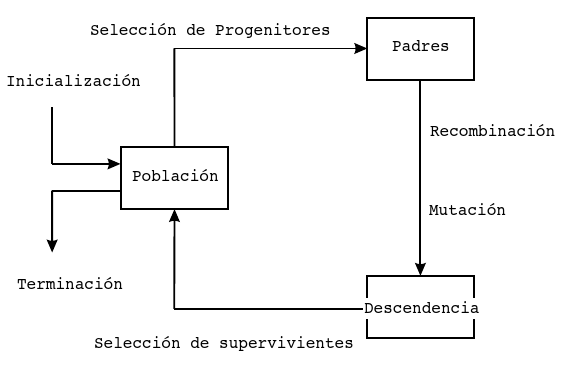
\includegraphics[scale=0.8,keepaspectratio=true]{./Figure1.png}
 \caption{Proceso de un algoritmo evolutivo. \cite{eiben2003introduction}} 
\end{figure}

Debido a que todas las variedades de algoritmos evolutivos siguen los lineamientos formulados tanto en el algoritmo est�ndar como en la Figura 3.1, las diferencias entre ellas se reducen a detalles t�cnicos, como la forma de representar las soluciones. Lo ideal es utilizar la representaci�n de datos m�s adecuada seg�n la naturaleza del problema a resolver. Si bien son varios los paradigmas desarrollados a partir de la computaci�n evolutiva, son tres los m�s importantes: Estrategias de Evoluci�n, Programaci�n Evolutiva y Algoritmos Gen�ticos, las cuales evolucionan soluciones para problemas parametrizados. A ellas se les sumar�a un cuarto paradigma: Programaci�n Gen�tica, el cual evoluciona los programas computacionales en s� con el fin de solucionar problemas computacionales \cite{kicinger2005evolutionary}.

Es necesario mencionar algunos conceptos propios de los algoritmos evolutivos, entre los cuales se encuentra al {\bf individuo} que es una soluci�n propuesta al problema; la {\bf poblaci�n} que es el conjunto de individuos a evaluar y evolucionar; la {\bf generaci�n} que es una iteraci�n del algoritmo en el que se eval�a la aptitud de los individuos de la poblaci�n para posteriormente obtener una poblaci�n nueva tras realizar cambios aplicando operadores tales como \textit{mutaci�n} o \textit{recombinaci�n}; el {\bf fenotipo} que son los rasgos observables de cada individuo; y el {\bf genotipo} que es la codificaci�n gen�tica factible de convertirse en un individuo.

Los algoritmos evolutivos emplean determinadas herramientas comunes en sus distintas variables:
\begin{itemize}
 \item Una forma de codificar las soluciones. Esta forma var�a de tal forma que podemos encontrar el uso de cadenas de alfabetos finitos como en los algoritmos gen�ticos, el de �rboles en la programaci�n evolutiva, o de vectores con valores reales en las estrategias evolutivas,entre otros \cite{kicinger2005evolutionary}
 \item Una funci�n de aptitud que depende tanto de los individuos como de la forma de evaluarlos. 
 \item Un mecanismo de selecci�n, el cual se basa en la aptitud.
 \item Un conjunto de operadores para reproducir y alterar a los individuos codificados.
\end{itemize}

Los algoritmos evolutivos poseen gran cantidad de aplicaciones, entre las que podemos contar problemas de optimizaci�n \cite{coello1999comprehensive} \cite{zhou2011multiobjective}, exploraci�n (arte evolutivo) \cite{romero2008art}, optimizaci�n de procesos qu�micos \cite{singulani2008computational}, entre muchos otros. Presentan gran cantidad de ventajas, entre las cuales podemos mencionar:
\begin{itemize}
 \item Aplicabilidad en problemas donde no hay otros m�todos disponibles, ya sea por presencia de restricciones no lineales, discontinuidad, multi-modalidad, problemas de ruido, etc.
 \item Adecuados para problemas que requieren m�ltiples soluciones, debido a la existencia de una poblaci�n de las mismas.
 \item Altamente paralelizables.
\end{itemize}

Por supuesto, los algoritmos evolutivos tambi�n presentan algunos inconvenientes, tales como: 
\begin{itemize}
 \item Los efectos que los errores del usuario pueden producir al momento de ajustar par�metros, los cuales pueden resultar en errores o en un desempe�o menor que �ptimo \cite{hinterding1997adaptation}.
 \item El ajuste de los par�metros puede tomar tiempo.
 \item El valor �ptimo de los par�metros pueden variar durante la evoluci�n.
 \item No existe una garant�a para hallar soluciones �ptimas en un periodo de tiempo determinado, aunque para evitar ello se pueden aplicar pruebas de convergencia asimpt�tica.
\end{itemize}






\section{Algoritmos Evolutivos de Inspiraci�n Cu�ntica}

Cada cap�tulo excepto el primero debe contener al finalizarlo una secci�n de consideraciones que enlacen
el presente cap�tulo con el siguiente.

\section{Consideraciones Finales}

Cada cap�tulo excepto el primero debe contener al finalizarlo una secci�n de consideraciones que enlacen
el presente cap�tulo con el siguiente.


 %Inserta el cap�tulo 3
\chapter{Propuesta}

Un cap�tulo puede contener n secciones. La referencia bibliogr�fica se hace de la siguiente manera:
\cite{zhang2011evolutionary}

En este cap�tulo se desarrolla toda la propuesta realizada a trav�s de la investigaci�n. Sigue la
misma estructura del cap�tulo anterior.

El t�tulo del cap�tulo es flexible de acuerdo a cada tesis. Algunos t�tulos sugeridos podr�an ser:

\begin{itemize}
\item El algoritmo X: nuestra propuesta.
\item La t�cnica Y
\end{itemize}

Este t�tulo debe de estar ade acuerdo con el asesor del tema. Cons�ltelo en su sala de clase. %Inserta el cap�tulo 4
\chapter{Pruebas y Resultados}

\section{Escenarios de prueba}

Como se indic� desde un principio, los escenarios para las pruebas son un conjunto de funciones \textit{benchmark} orientadas a problemas de optimizaci�n de objetivo �nico especialmente seleccionadas para evaluar el desempe�o de los algoritmos derivados comparativamente con respecto al algoritmo original. Las funciones fueron seleccionadas a partir de \cite{mishra2006some} \cite{silagadze2007finding}.

\begin{table}[h]
\begin{tabularx}{\textwidth}{ |X|X|X|X| }
\hline
Funci�n			& F�rmula 		& Valor m�nimo		& Dominio de b�squeda \\ \hline
Funci�n de Arckley	& No			& No			& No   \\
Funci�n de Booth   	& No			& No			& No   \\
Funci�n de Maytas   	& No			& No			& No   \\
\hline
\end{tabularx}
\caption{Descripci�n de las funciones de prueba}
 \label{table5-1}
\end{table}

\begin{figure}
   \centering
    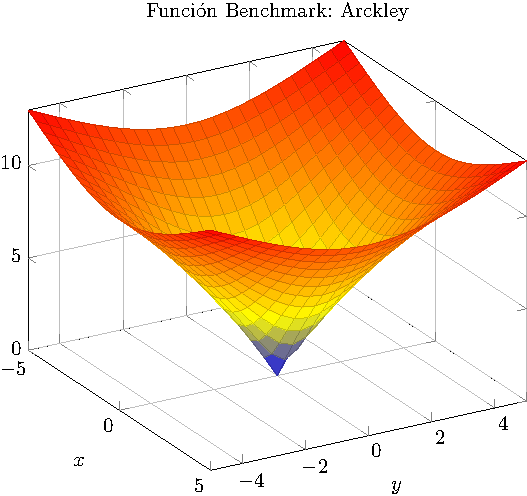
\includegraphics{./Figures/Functions/arckley.pdf}%
   \caption{Funci�n Benchmark: Arckley}
   \label{figure5-1}
\end{figure}

\begin{figure}
   \centering
    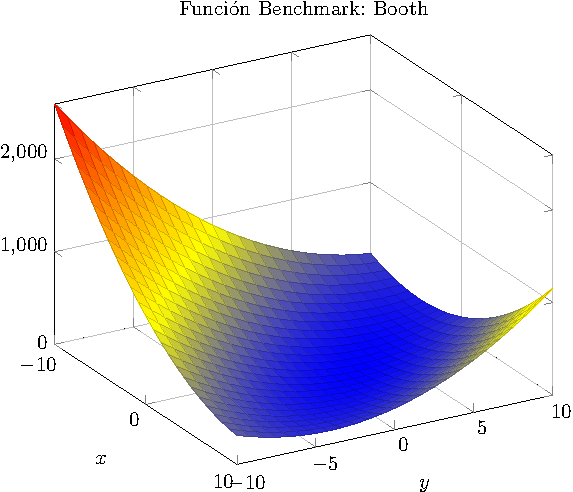
\includegraphics{./Figures/Functions/booth.pdf}%
   \caption{Funci�n Benchmark: Booth}
   \label{figure5-8}
\end{figure}

\begin{figure}
   \centering
    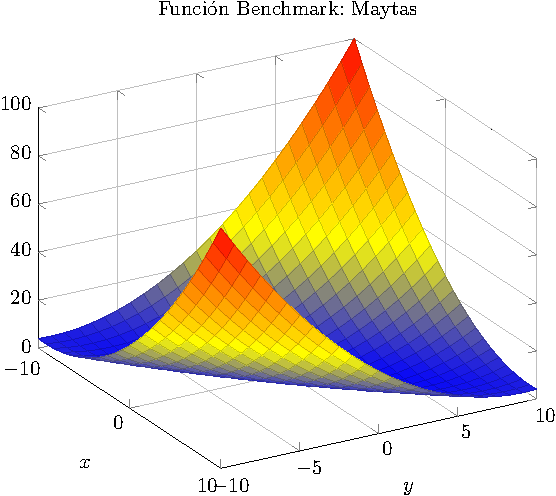
\includegraphics{./Figures/Functions/maytas.pdf}%
   \caption{Funci�n Benchmark: Maytas}
   \label{figure5-15}
\end{figure}



\section{Condiciones para las pruebas}

\section{Resultados}

\subsection{}
\subsection{}
\subsection{}
\subsection{}
\subsection{}
\subsection{}

The path of the righteous man is beset on all sides by the iniquities of the selfish and the tyranny of evil men. Blessed is he who, in the name of charity and good will, shepherds the weak through the valley of darkness, for he is truly his brother's keeper and the finder of lost children. And I will strike down upon thee with great vengeance and furious anger those who would attempt to poison and destroy My brothers. And you will know My name is the Lord when I lay My vengeance upon thee fdgsdfss.

Now that there is the Tec-9, a crappy spray gun from South Miami. This gun is advertised as the most popular gun in American crime. Do you believe that shit? It actually says that in the little book that comes with it: the most popular gun in American crime. Like they're actually proud of that shit. 

The path of the righteous man is beset on all sides by the iniquities of the selfish and the tyranny of evil men. Blessed is he who, in the name of charity and good will, shepherds the weak through the valley of darkness, for he is truly his brother's keeper and the finder of lost children. And I will strike down upon thee with great vengeance and furious anger those who would attempt to poison and destroy My brothers. And you will know My name is the Lord when I lay My vengeance upon thee fdgsdfss.

Now that there is the Tec-9, a crappy spray gun from South Miami. This gun is advertised as the most popular gun in American crime. Do you believe that shit? It actually says that in the little book that comes with it: the most popular gun in American crime. Like they're actually proud of that shit. 

The path of the righteous man is beset on all sides by the iniquities of the selfish and the tyranny of evil men. Blessed is he who, in the name of charity and good will, shepherds the weak through the valley of darkness, for he is truly his brother's keeper and the finder of lost children. And I will strike down upon thee with great vengeance and furious anger those who would attempt to poison and destroy My brothers. And you will know My name is the Lord when I lay My vengeance upon thee fdgsdfss.

Now that there is the Tec-9, a crappy spray gun from South Miami. This gun is advertised as the most popular gun in American crime. Do you believe that shit? It actually says that in the little book that comes with it: the most popular gun in American crime. Like they're actually proud of that shit. 


\begin{figure}
   \centering
    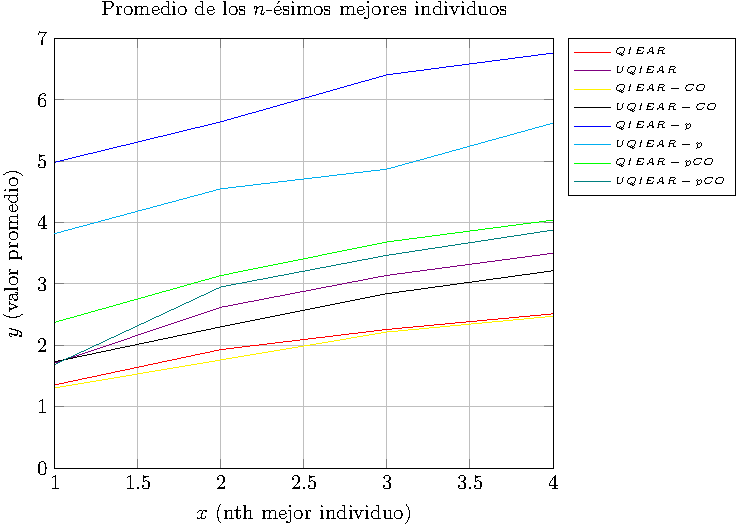
\includegraphics{./Figures/arckley_nth_cind2.pdf}%
   \caption{Valor promedio de los $n$-�simos mejores individuos para $ci=2$}
   \label{figure5-2}
\end{figure}

\begin{figure}
   \centering
    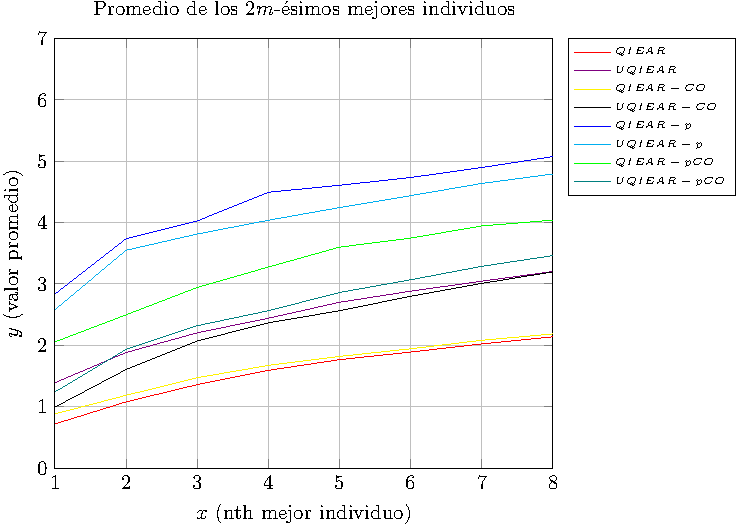
\includegraphics{./Figures/arckley_nth_cind4.pdf}%
   \caption{Valor promedio de los $n$-�simos mejores individuos para $ci=4$}
   \label{figure5-3}
\end{figure}

\begin{figure}
   \centering
    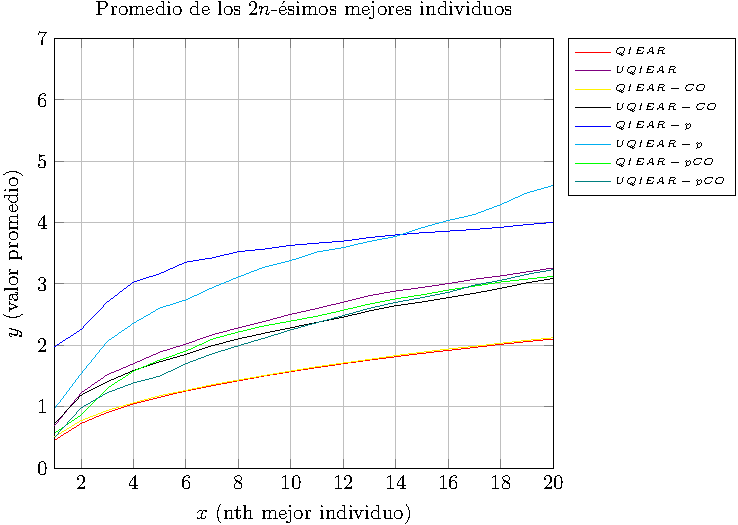
\includegraphics{./Figures/arckley_nth_cind10.pdf}%
   \caption{Valor promedio de los $n$-�simos mejores individuos para $ci=10$}
   \label{figure5-4}
\end{figure}

\begin{figure}
   \centering
    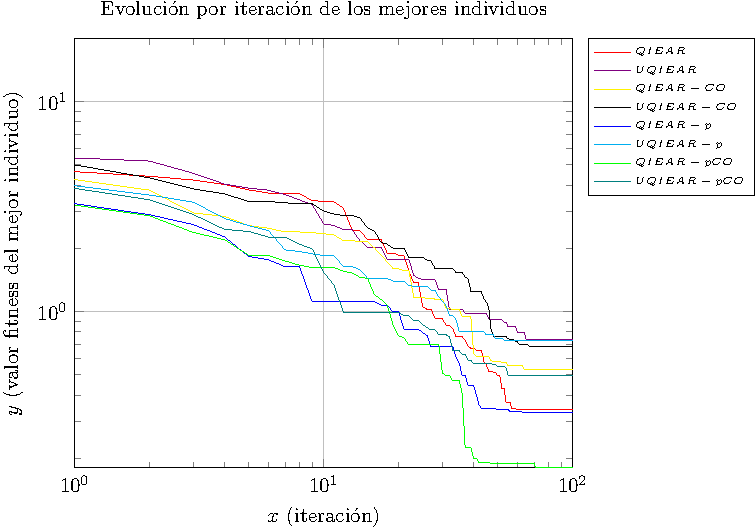
\includegraphics{./Figures/arckley_bestevol_cind3.pdf}%
   \caption{Evoluci�n de los valores de los mejores individuos para $ci=3$}
   \label{figure5-5}
\end{figure}

\begin{figure}
   \centering
    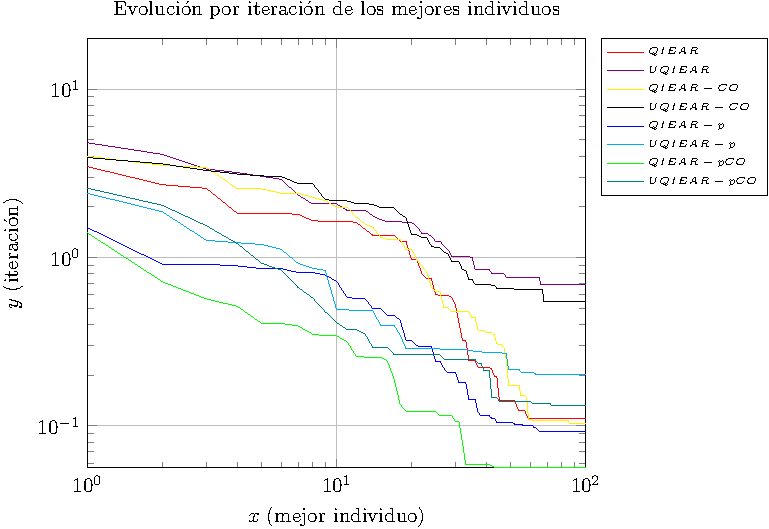
\includegraphics{./Figures/arckley_bestevol_cind7.pdf}%
   \caption{Evoluci�n de los valores de los mejores individuos para $ci=7$}
   \label{figure5-6}
\end{figure}

\begin{figure}
   \centering
    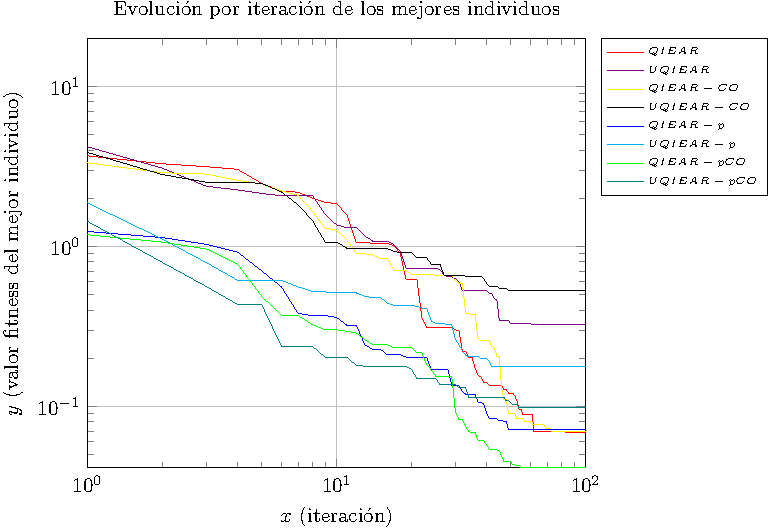
\includegraphics{./Figures/arckley_bestevol_cind9.pdf}%
   \caption{Evoluci�n de los valores de los mejores individuos para $ci=9$}
   \label{figure5-7}
\end{figure}

The path of the righteous man is beset on all sides by the iniquities of the selfish and the tyranny of evil men. Blessed is he who, in the name of charity and good will, shepherds the weak through the valley of darkness, for he is truly his brother's keeper and the finder of lost children. And I will strike down upon thee with great vengeance and furious anger those who would attempt to poison and destroy My brothers. And you will know My name is the Lord when I lay My vengeance upon thee fdgsdfss.

Now that there is the Tec-9, a crappy spray gun from South Miami. This gun is advertised as the most popular gun in American crime. Do you believe that shit? It actually says that in the little book that comes with it: the most popular gun in American crime. Like they're actually proud of that shit. 

The path of the righteous man is beset on all sides by the iniquities of the selfish and the tyranny of evil men. Blessed is he who, in the name of charity and good will, shepherds the weak through the valley of darkness, for he is truly his brother's keeper and the finder of lost children. And I will strike down upon thee with great vengeance and furious anger those who would attempt to poison and destroy My brothers. And you will know My name is the Lord when I lay My vengeance upon thee fdgsdfss.

Now that there is the Tec-9, a crappy spray gun from South Miami. This gun is advertised as the most popular gun in American crime. Do you believe that shit? It actually says that in the little book that comes with it: the most popular gun in American crime. Like they're actually proud of that shit. 

The path of the righteous man is beset on all sides by the iniquities of the selfish and the tyranny of evil men. Blessed is he who, in the name of charity and good will, shepherds the weak through the valley of darkness, for he is truly his brother's keeper and the finder of lost children. And I will strike down upon thee with great vengeance and furious anger those who would attempt to poison and destroy My brothers. And you will know My name is the Lord when I lay My vengeance upon thee fdgsdfss.

Now that there is the Tec-9, a crappy spray gun from South Miami. This gun is advertised as the most popular gun in American crime. Do you believe that shit? It actually says that in the little book that comes with it: the most popular gun in American crime. Like they're actually proud of that shit. 


\begin{figure}
   \centering
    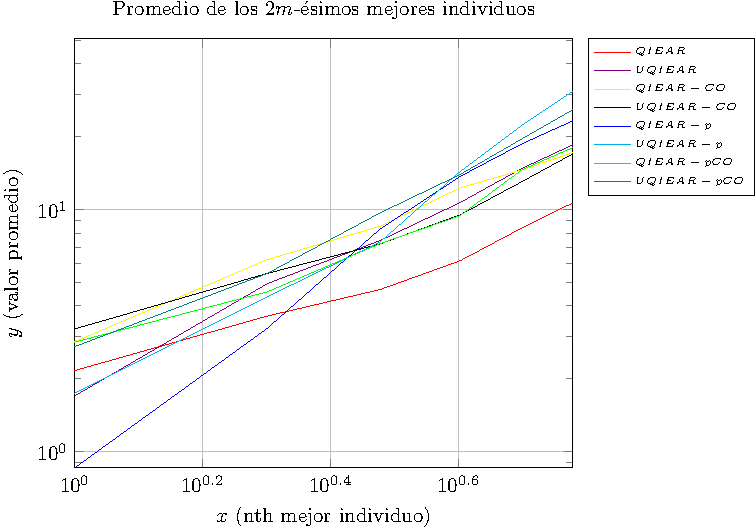
\includegraphics{./Figures/booth_nthbest_cind3.pdf}%
   \caption{Valor promedio de los $n$-�simos mejores individuos para $ci=3$}
   \label{figure5-9}
\end{figure}

\begin{figure}
   \centering
    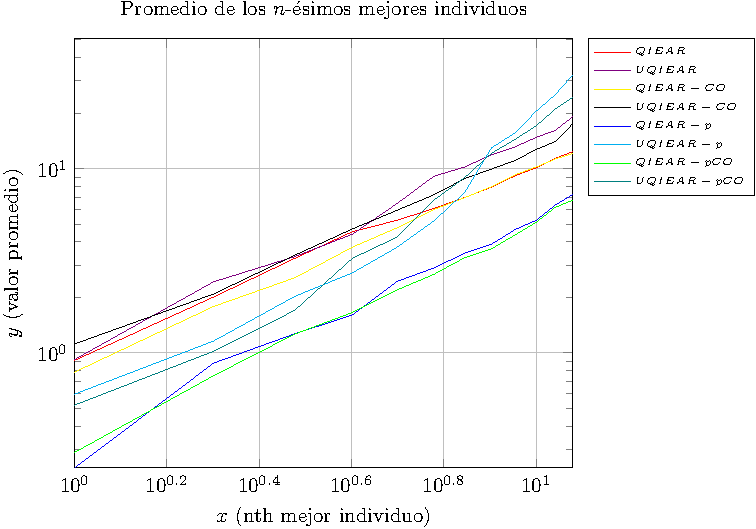
\includegraphics{./Figures/booth_nthbest_cind6.pdf}%
   \caption{Valor promedio de los $n$-�simos mejores individuos para $ci=6$}
   \label{figure5-10}
\end{figure}

\begin{figure}
   \centering
    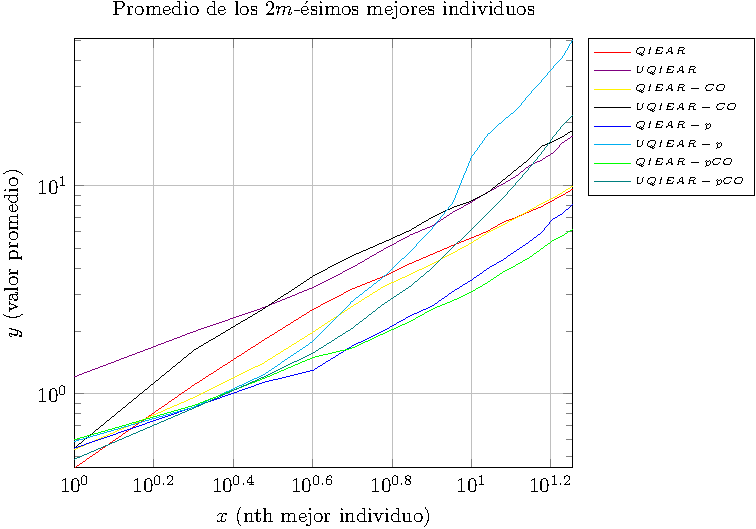
\includegraphics{./Figures/booth_nthbest_cind9.pdf}%
   \caption{Valor promedio de los $n$-�simos mejores individuos para $ci=9$}
   \label{figure5-11}
\end{figure}

\begin{figure}
   \centering
    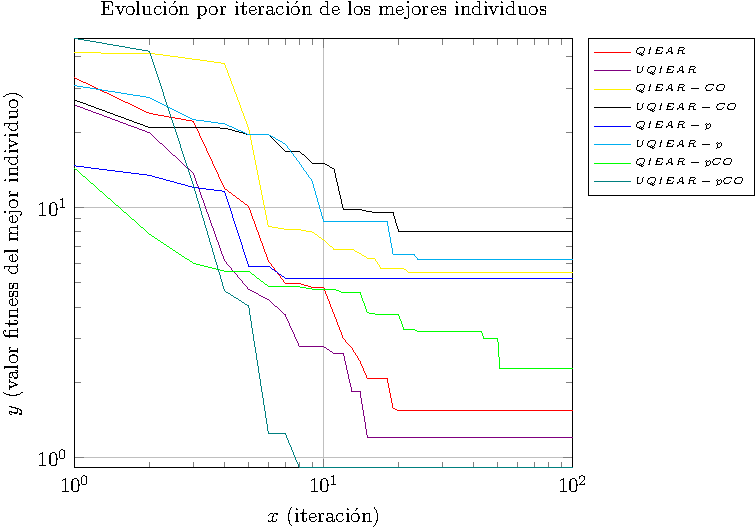
\includegraphics{./Figures/booth_bestevol_cind2.pdf}%
   \caption{Evoluci�n de los valores de los mejores individuos para $ci=2$}
   \label{figure5-12}
\end{figure}

\begin{figure}
   \centering
    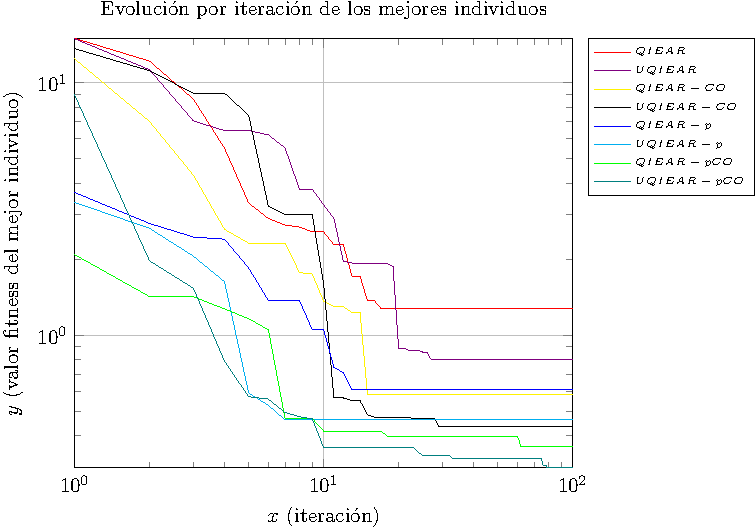
\includegraphics{./Figures/booth_bestevol_cind4.pdf}%
   \caption{Evoluci�n de los valores de los mejores individuos para $ci=4$}
   \label{figure5-13}
\end{figure}

\begin{figure}
   \centering
    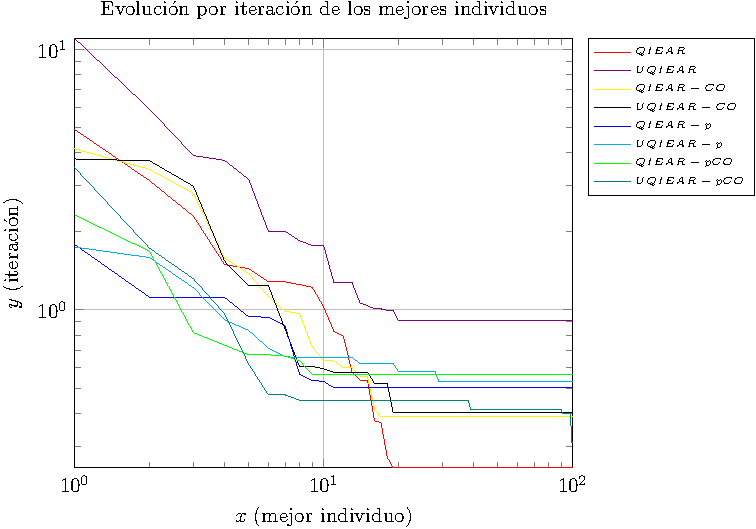
\includegraphics{./Figures/booth_bestevol_cind9.pdf}%
   \caption{Evoluci�n de los valores de los mejores individuos para $ci=9$}
   \label{figure5-14}
\end{figure}

The path of the righteous man is beset on all sides by the iniquities of the selfish and the tyranny of evil men. Blessed is he who, in the name of charity and good will, shepherds the weak through the valley of darkness, for he is truly his brother's keeper and the finder of lost children. And I will strike down upon thee with great vengeance and furious anger those who would attempt to poison and destroy My brothers. And you will know My name is the Lord when I lay My vengeance upon thee fdgsdfss.

Now that there is the Tec-9, a crappy spray gun from South Miami. This gun is advertised as the most popular gun in American crime. Do you believe that shit? It actually says that in the little book that comes with it: the most popular gun in American crime. Like they're actually proud of that shit. 

The path of the righteous man is beset on all sides by the iniquities of the selfish and the tyranny of evil men. Blessed is he who, in the name of charity and good will, shepherds the weak through the valley of darkness, for he is truly his brother's keeper and the finder of lost children. And I will strike down upon thee with great vengeance and furious anger those who would attempt to poison and destroy My brothers. And you will know My name is the Lord when I lay My vengeance upon thee fdgsdfss.

Now that there is the Tec-9, a crappy spray gun from South Miami. This gun is advertised as the most popular gun in American crime. Do you believe that shit? It actually says that in the little book that comes with it: the most popular gun in American crime. Like they're actually proud of that shit. 

The path of the righteous man is beset on all sides by the iniquities of the selfish and the tyranny of evil men. Blessed is he who, in the name of charity and good will, shepherds the weak through the valley of darkness, for he is truly his brother's keeper and the finder of lost children. And I will strike down upon thee with great vengeance and furious anger those who would attempt to poison and destroy My brothers. And you will know My name is the Lord when I lay My vengeance upon thee fdgsdfss.

Now that there is the Tec-9, a crappy spray gun from South Miami. This gun is advertised as the most popular gun in American crime. Do you believe that shit? It actually says that in the little book that comes with it: the most popular gun in American crime. Like they're actually proud of that shit. 

\begin{figure}
   \centering
    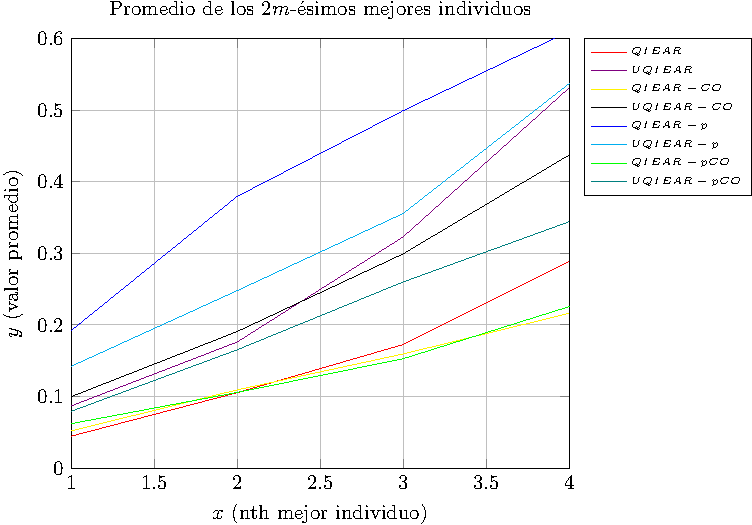
\includegraphics{./Figures/maytas_nthbest_cind2.pdf}%
   \caption{Valor promedio de los $n$-�simos mejores individuos para $ci=2$}
   \label{figure5-16}
\end{figure}

\begin{figure}
   \centering
    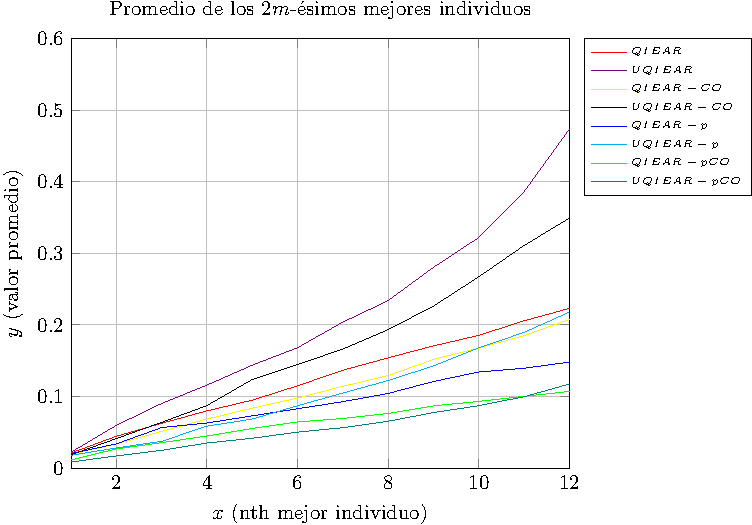
\includegraphics{./Figures/maytas_nthbest_cind6.pdf}%
   \caption{Valor promedio de los $n$-�simos mejores individuos para $ci=6$}
   \label{figure5-17}
\end{figure}

\begin{figure}
   \centering
    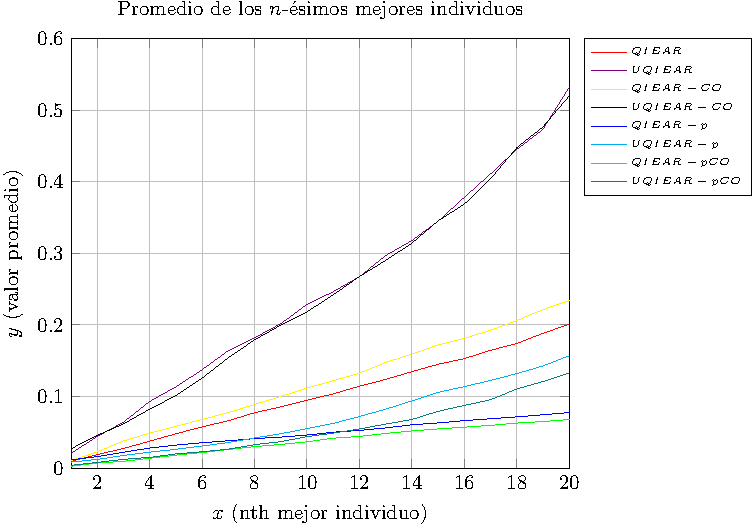
\includegraphics{./Figures/maytas_nthbest_cind10.pdf}%
   \caption{Valor promedio de los $n$-�simos mejores individuos para $ci=10$}
   \label{figure5-18}
\end{figure}

\begin{figure}
   \centering
    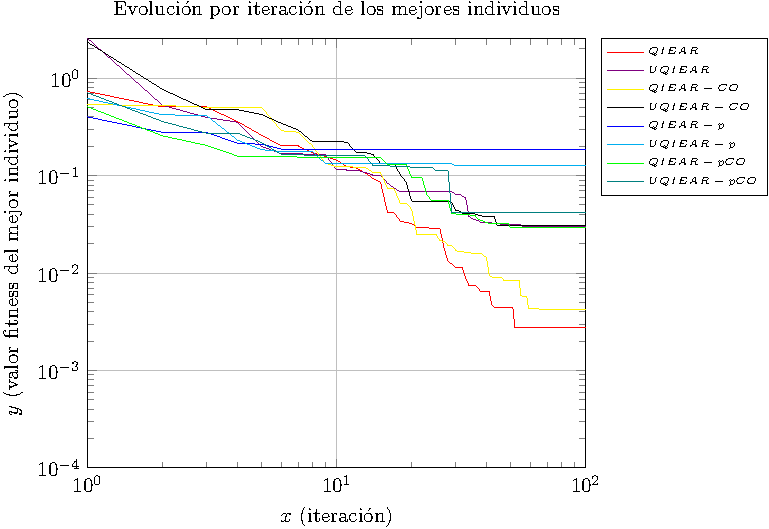
\includegraphics{./Figures/maytas_bestevol_cind2.pdf}%
   \caption{Evoluci�n de los valores de los mejores individuos para $ci=2$}
   \label{figure5-19}
\end{figure}

\begin{figure}
   \centering
    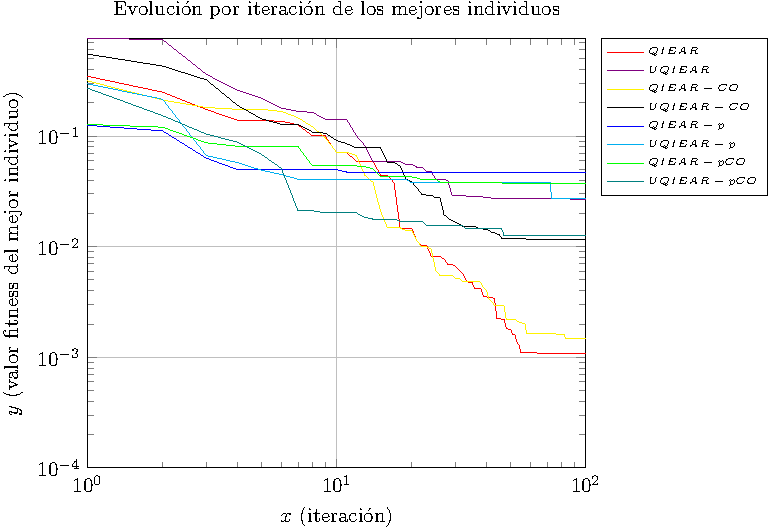
\includegraphics{./Figures/maytas_bestevol_cind4.pdf}%
   \caption{Evoluci�n de los valores de los mejores individuos para $ci=4$}
   \label{figure5-20}
\end{figure}

\begin{figure}
   \centering
    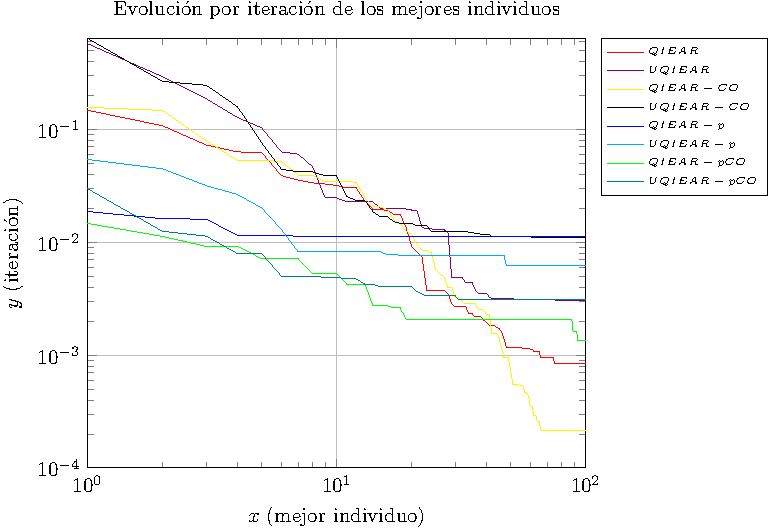
\includegraphics{./Figures/maytas_bestevol_cind10.pdf}%
   \caption{Evoluci�n de los valores de los mejores individuos para $ci=10$}
   \label{figure5-21}
\end{figure}


 %Inserta el cap�tulo 5
\chapter{Conclusiones y Trabajos Futuros}\label{chap:conclusiones}

El presente trabajo ha propuesto distintas modificaciones al algoritmo original \ac{QIEA}$\mathbb{R}$ con la expectativa por obtener resultados mejores en t�rminos de tiempo de convergencia y calidad de datos generados. En t�rminos generales, los �nicos algoritmos que han registrado resultados medianamente consistentes y competitivos en t�rminos de rapidez de convergencia as� como de calidad de datos a lo largo de todas las pruebas son las variantes que implementan el operador de recombinaci�n en espacios particionados. Esto es: \ac{QIEA}$\mathbb{R}$-pCO y U\ac{QIEA}$\mathbb{R}$-pCO. Ambos han logrado obtener resultados mejores que los algoritmos originales (\ac{QIEA}$\mathbb{R}$ y \ac{QIEA}$\mathbb{R}$-p), en casos donde el n�mero de individuos cl�sicos generados por individuo cu�ntico por iteraci�n es m�s bajo. Cuando el n�mero de individuos cl�sicos aumenta, los algoritmos originales terminan comportandose de una manera m�s eficiente. Por lo tanto, se puede concluir que el operador de recombinaci�n propuesto es una alternativa v�lida que reduce la necesidad de generar una cantidad alta de individuos cl�sicos.

Por otro lado, los algoritmos que implementan la segregaci�n en los campos de operaci�n de cada individuo cl�sico no manifiestan una diferencia sustancial que permita distinguirlos de sus contrapartes no segregadas. En los casos en los que un algoritmo con espacios de b�squeda segregados por individuo cu�ntico destaca -U\ac{QIEA}$\mathbb{R}$-pCO es un buen ejemplo de este caso-, parece ser m�s influencia del propio operador de recombinaci�n que de la segregaci�n propiamente dicha.

Los dem�s algoritmos propuestos obtuvieron resultados m�s irregulares y menos �ptimos, por lo que se desaconseja su consideraci�n a futuro. Cabe destacar que los algoritmos con peores resultados en general fueron los que implementaban el particionamiento del espacio de b�squeda sin el operador de recombinaci�n.

\section{Problemas encontrados}
Un problema inherente al propio desarrollo de la presente tesis es la propia tendencia del algoritmo a sobreincrementar r�pidamente sus espacios de b�squeda tras un espacio de tiempo en el que no se hallan mejores soluciones, por lo que las propuestas no se han podido evaluar para problemas con espacios de b�squeda mayores a los escogidos en el presente trabajo.

Las pruebas en funciones con m�nimos ubicados cercanos en los extremos de los espacios de b�squeda tambi�n han representado un reto que no se pudo asumir, debido a la inexistencia de una metodolog�a apropiada para la delimitaci�n de la expansi�n en el espacio de b�squeda del algoritmo original, y por tanto, tampoco en los aqu� propuestos. El comportamiento del algoritmo lo impulsa a buscar m�s m�nimos fuera de dichos l�mites, por lo que terminar�an tendiendo hacia un m�nimo no contemplado al interior del espacio de b�squeda. 

%\section{Recomendaciones}

\section{Trabajos futuros}
Para futuras evaluaciones, se planea tomar en consideraci�n la implementaci�n de otras metodolog�as tanto para la actualizaci�n de los individuos cu�nticos como para la propia selecci�n de los mejores individuos cl�sicos. De esta manera, se tendr�a un conjunto m�s amplio de situaciones sobre las cuales evaluar a los algoritmos aqu� propuestos.

Se vislumbra como posibilidad como complemento para el actual trabajo la ejecuci�n de pruebas sobre funciones multiobjetivo, en las que se evaluar�a no solamente la convergencia hacia un m�nimo o m�ximo, sino tambi�n la detecci�n de la ocurrencia de la convergencia hacia cada �ptimo por separado.  %Inserta el cap�tulo 6

%%%%%%%%%%%%%%%%%%%%%%%%%%%%%%%%%%%%%%%%%%%%%%%%%%%%%%%%%%%%%%%%%%%%%%

\bibliographystyle{apalike}
\bibliography{Bibliog}
\addcontentsline{toc}{chapter}{Bibliograf�a}
\end{document}
